\documentclass[journal]{IEEEtran}

\usepackage{blindtext}
\usepackage{graphicx}
\usepackage{cite}
\usepackage[utf8x]{inputenc}
\usepackage[slovene,english]{babel}  
\usepackage{url}

\hyphenation{op-tical net-works semi-conduc-tor}
\begin{document}
\title{IMapBooks - Automatic Question Response Grading}
\author{Tilen Tomakić\\tt5157@student.uni-lj.si\\https://github.com/TilenTomakic/IMapBooks-AQRG\\https://hub.docker.com/r/tilen/sag}%
\maketitle

%  Abstract -  summary of problem and contribution
\begin{abstract}	
  Dokument opisuje raziskavo metod mapiranja, ekstrakcije informacij in uporabe korpusa za točkovanje pravilnosti odgovorov na vprašanja iz podane zgodbe. Uporabljeni so bili tri pristopi (metode). Od osnovnega do naprednejšega.
\end{abstract}

\begin{IEEEkeywords}
NLP, IMapBook, SAG, CAM
\end{IEEEkeywords}

\IEEEpeerreviewmaketitle

% Introduction - problem motivation and background
\section{Uvod}
V angleščini problemsko domeno imenujemo "Short Answer Grading (SAG)". SAG se ukvarja z ocenjevanjem krajših odgovorov (2-3 stavki).

Cilj je bil raziskati tehnike ovrednotenja pravilnosti odgovorov. Pri ovrednotenju je že na voljo množica ovrednotenih odgovorov na enaka vprašanja. Odgovori odgovarjajo na vprašanja podana iz besedila oz. zgodbe.

Problem zaznave pravilih in napačnih odgovorov nam lahko pomaga tudi pri širših problemskih domenah, kot so zaznava lažnih novic.\\

Raziskava je bila osnovana na podatkovni množici vprašanj in odgovor iz IMapBook (\textit{https://www.imapbook.com/}) vira. V množici, sta dva učitelja ovrednotila odgovore učencev na temo prebrane zgodbe. Odgovori so ovrednoteni s 0, 0,5 ali 1 točko.\\

Opisani so tri pristopi reševanja problema. Modeli A, B in C. Enako kot učitelja modeli ovrednotijo odgovore s točkami 0, 0,5 ali 1. Modeli so bili spisani s ciljem neodvisnosti od poznavanja tematike domene, s tem jih je mogoče uporabiti ne le v primeru zgodb.

%  Related work - relevant literature overview
\section{Podobna dela}
Obstaja več strategij oz. kombinacij reševanja problem a ocenjevanja~\cite{adhya2016automated}.
Strategije delimo na slikanje koncepta (angl. concept mapping), ekstrakcija informacij (angl. information extraction), metode s pomočjo korpusov (angl. corpus-based methods), strojno učenje (angl. machine learning) in vrednotenje (angl. evaluation).

Podobni deli temu dokumentu sta CAM (angl. Content Assessment Module)~\cite{bailey2008content} in delo Ulrike Pado in Cornelia Kiefer~\cite{Kiefer}.\\

CAM pristop integrira več strategij ujemanja na različnih stopnjah obdelanega besedila. Na ta način primerja in oceni pomen odgovora.
Na splošno CAM primerja odgovor z znano bazo odgovorov in ugotovi ali odgovor vsebuje enak semantični pomen~\cite{bailey2008diagnosing}.\\

Delo Ulrike Pado in Cornelia z angl. naslovom \textit{Short Answer Grading: When Sorting Helps and When it Doesn’t} je najbolj podobno modeloma B in C opisana v tem dokumentu. Kot glavno komponento sta avtorja uporabila binarno klasifikacijo. Rezultati uspešnosti so primerljivi z ugotovitvami pri C modelu (testna množica IMapBook vprašanja in odgovori).

%  Methods - used methods and techniques
\section{Uporabljene metode}
Uporabljene so bile 3 metode, s ciljem primerjanja rezultatov med njimi. Pričakovan rezultat je bil, da se modela A izkaže kot slaba metoda, model C pa najboljša.

\subsection{Model A}
Model A na začetku izvajanja algoritma izbere en odgovor iz znane množice pravilnih. Odloči se na podlagi kriterija najpopolnejšega odgovora. Najpopolnejši odgovor je določen na podlagi:
\begin{itemize}
	\item Odgovor, ki ima večje število besed.
	\item Število tem v odgovoru. Za pridobitev abstraktnih tem  v odgovoru je bil uporabljen LDA (angl. Latent Dirichlet allocation) algoritem.
\end{itemize}

Izbran odgovor je uporabljen za ocenjevaje drugih. Pred testiranjem odgovora so besede najprej pretvorjene v njihove osnovne korene s pomočjo "Porter stemmer" algoritma. Več besed testiranega odgovora se ujema s pred izbranim večja je verjetnost, da je ocenjevan odgovor pravilen. Potek viden na sliki~\ref{sl:ma}. 

Faktor za določitev ocene 1 je bil nastavljen na 10\%. Majhna konstanta je bil nastavljena zato, ker so iz odgovorov že pred primerjavo odstranjene zaustavljive besede (stop words). Zato je že majhno ujemanje besed dovolj za oceno 0,5 oz. 1.

\begin{figure}[h]
	\centering
	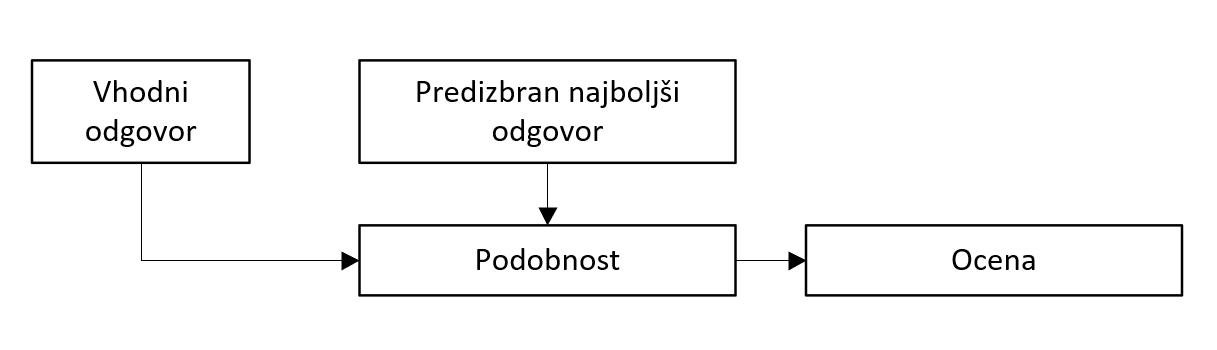
\includegraphics[width=3.5in]{A}
	\caption{Diagram poteka za model A}
	\label{sl:ma}
\end{figure}

\subsection{Model B}
Model B je podoben modelu A, vendar se ne odloči za statičen odgovor na začetku. Pravilnost odgovora testira nad celotno znano množico odgovorov. Ker ima B model na voljo celotno množico odgovor, je bila uporabljena binarna klasifikacija. Diagram poteka viden na sliki~\ref{sl:mb}. F1 micro rezultat pri poganjaju "cross validation" je 84,13\%.

\begin{figure}[h]
	\centering
	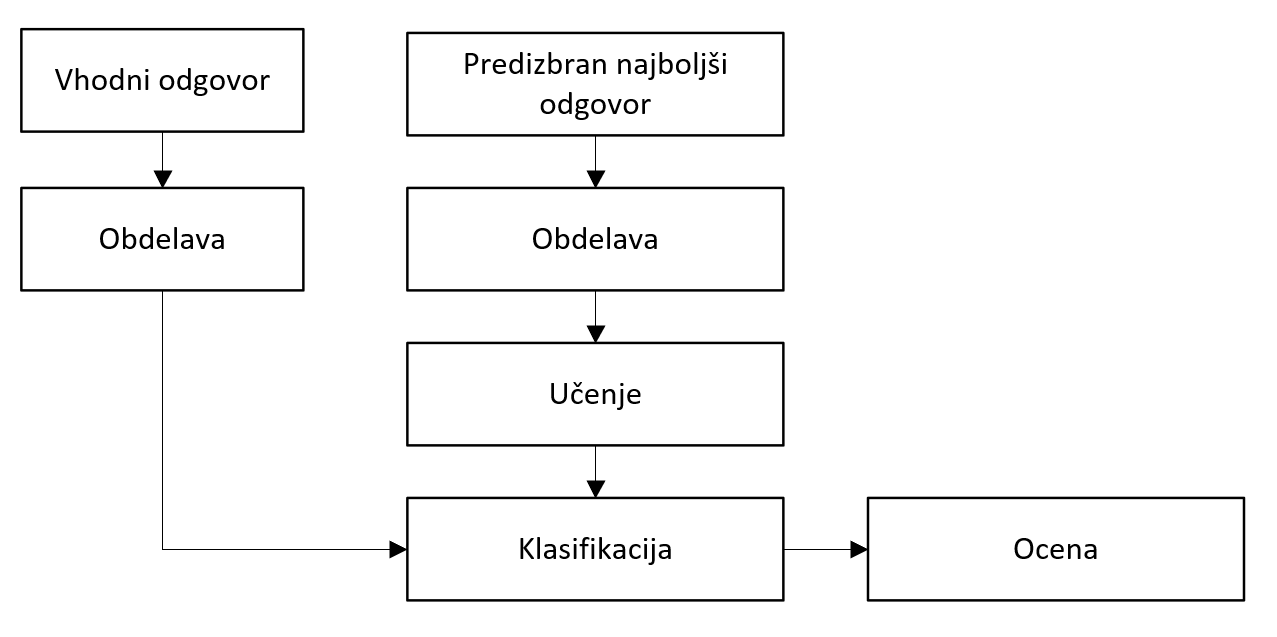
\includegraphics[width=3.4in]{B}
	\caption{Model B shema}
	\label{sl:mb}
\end{figure}

\subsection{Model C}
Model C je nadgradnja modela B. Pred učenjem klasifikatorja je bil uporabljen zunanji vir sopomenk. Najprej je bil uporabljen concept net API. Vendar zaradi omejitev API-ja je bila uporabljena lokalna baza sopomenk s pomočjo npm knjižnice "synonyms". Diagram poteka viden na sliki~\ref{sl:mc}.

Tu je bil cilj besede poenostaviti na enake imenovalce. Pri prvem poskusu so bili sinonimi direktno dodani v klasifikator. To je povzročilo slabše rezultate (F1 micro 25\%). Zato sem vse besede, ki imajo enako skupino sinonimov zamenjal le z enim sinonimom (vedno enakim). To je popravilo drastično slabše rezultate, vendar so rezultati še vedno za 2\% slabši kot pri modelu B.

\begin{figure}[h]
	\centering
	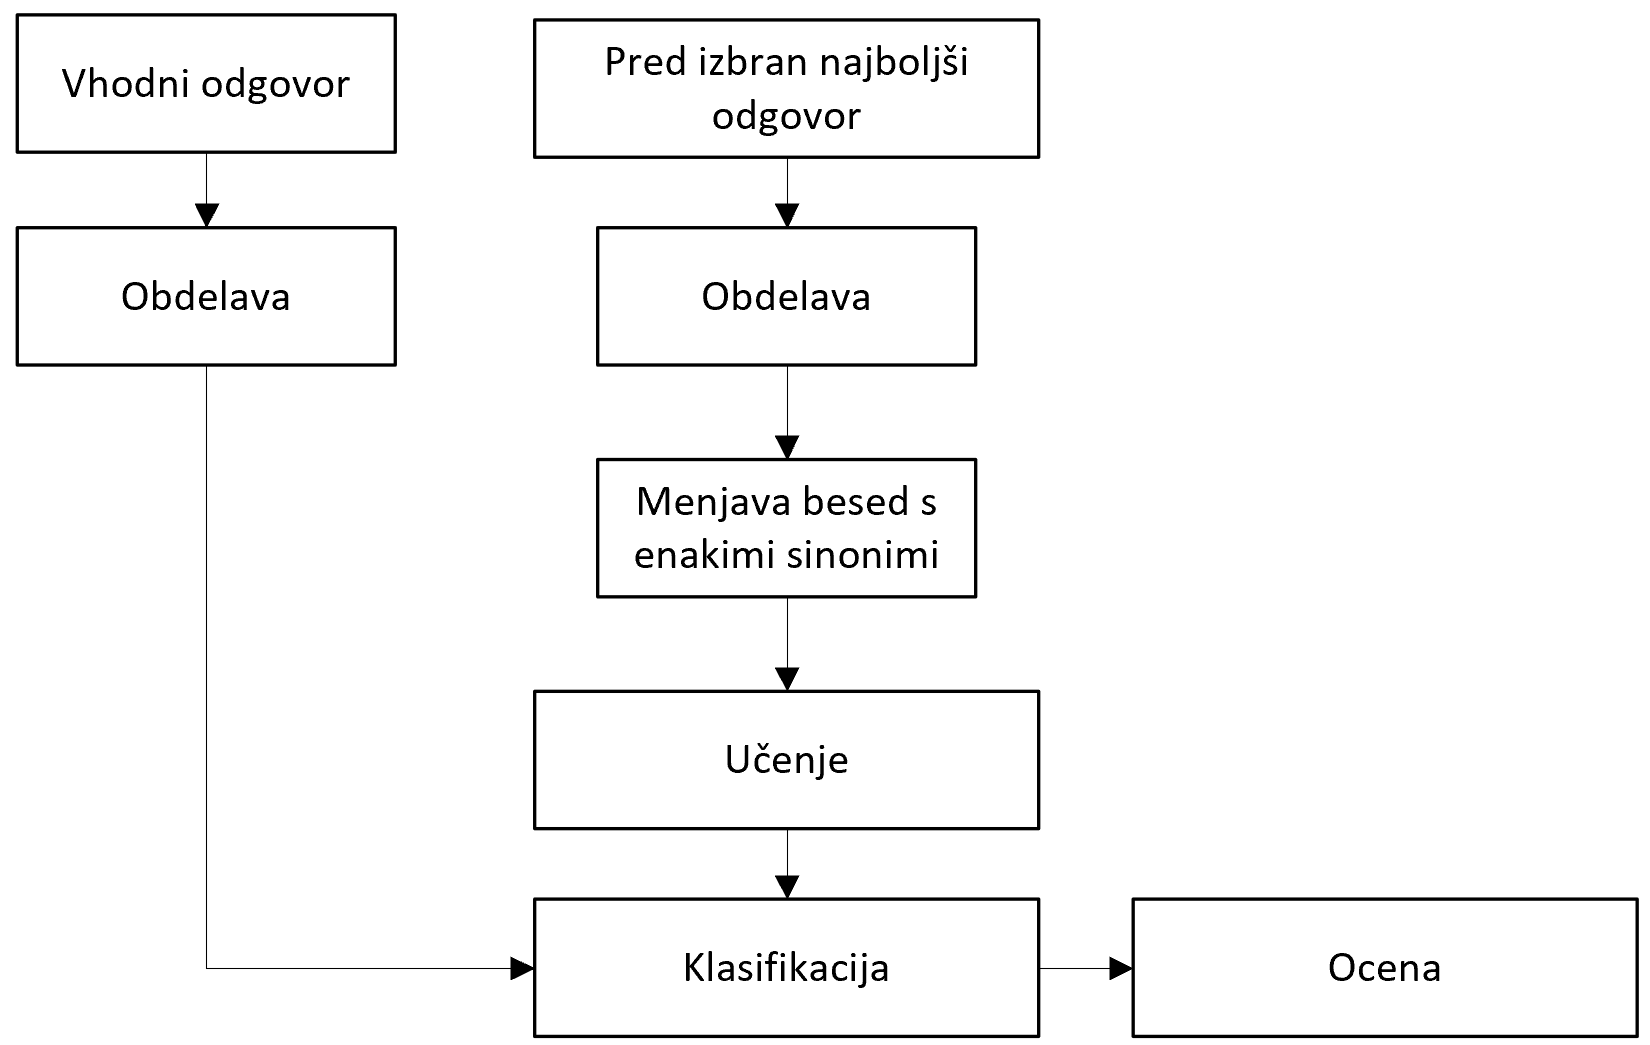
\includegraphics[width=3.4in]{C}
	\caption{Model C shema}
	\label{sl:mc}
\end{figure}

% Results - results description
% Discussion - results comparison and evaluation
\section{Rezultati}
Uspešnosti modelov po posameznih skupinah vprašanj je vidna na tabeli~\ref{t:mod}. Zanimivo je, da so rezulati uspešnosti modelov drugačni od pričakovanih. V povprečju (F1 micro) se je model B izkazal kot boljši. Pri vseh razen dveh skupinah vprašanj je C model z uporabo dodatnih virov dosegel slabši rezultat.

Slabše rezultate pripisujem temu, da so določene besede znotraj odgovora bile spremenjene na enak imenovalec, čeprav ta zamenjav ni bila najboljša.

\begin{table}[]
	\begin{tabular}{l|l|l|l|}
		\cline{2-4}
		                            & Model A          & Model B          & Model C          \\ \hline


	
	\multicolumn{1}{|l|}{How does Shiranna feel as t...} & \textbf{60.49\%} & \textbf{91.25\%} & \textbf{92.50\%} \\ \hline
	\multicolumn{1}{|l|}{Why did her body want to fl...} & \textbf{64.20\%} & \textbf{73.75\%} & \textbf{72.50\%} \\ \hline
	\multicolumn{1}{|l|}{Why do Adam cheeks “flush”?} & \textbf{78.57\%} & \textbf{90.00\%} & \textbf{91.43\%} \\ \hline
	\multicolumn{1}{|l|}{Why is the door locked?} & \textbf{84.87\%} & \textbf{78.67\%} & \textbf{76.00\%} \\ \hline
	\multicolumn{1}{|l|}{Why does Shiranna’s father ...} & \textbf{57.46\%} & \textbf{63.08\%} & \textbf{63.08\%} \\ \hline
	\multicolumn{1}{|l|}{How do you think Shiranna’s...} & \textbf{80.43\%} & \textbf{73.85\%} & \textbf{66.15\%} \\ \hline
	\multicolumn{1}{|l|}{Why is every adult trying t...} & \textbf{57.04\%} & \textbf{98.57\%} & \textbf{98.57\%} \\ \hline
	\multicolumn{1}{|l|}{What causes seasons to occu...} & \textbf{94.20\%} & \textbf{90.77\%} & \textbf{89.23\%} \\ \hline
	\multicolumn{1}{|l|}{How does Shiranna feel abou...} & \textbf{75.00\%} & \textbf{78.33\%} & \textbf{76.67\%} \\ \hline
	\multicolumn{1}{|l|}{What is happening in the tu...} & \textbf{84.62\%} & \textbf{84.62\%} & \textbf{81.54\%} \\ \hline
	\multicolumn{1}{|l|}{How does Adam’s family stru...} & \textbf{94.12\%} & \textbf{93.85\%} & \textbf{93.85\%} \\ \hline
	\multicolumn{1}{|l|}{Will the journey to Venus w...} & \textbf{81.69\%} & \textbf{92.86\%} & \textbf{91.43\%} \\ \hline
	\multicolumn{1}{|l|}{Skupaj} & \textbf{63.76\%} & \textbf{84.13\%} & \textbf{82.75\%} \\ \hline
		
		
	\end{tabular}
	\caption{Uspešnost modelov F1 micro score}
	\label{t:mod}
\end{table}

Medsebojni dogovor (\textit{angl. inter-rater agreemen}) ocene ocenjevalcev je bil izračunan po algoritmu Cohen's kappa. Rezultat medsebojnega dogovora je 73\%.

\section{Zaključek}
Že v sami IMapBook množici, se dva ocenjevalca pri vseh odgovorih nista strinjala o njihovi oceni. Pri ocenjevanju je računalniški algoritem lahko le tako dober kot je človek. Če se človek ne more strinjati o oceni, je težko pričakovati, da bo algoritem opravil boljše.\\

Pri odgovorih je pomembno, da algoritem prepozna ključne besede. Če so ključne besede filtrirane so lahko rezultati napačni. Iz tega razloga sem tudi izklopil TF-IDF metodo oteževanja besed, saj so se oteži izkazale za napačne. Kot posledica je klasifikator napačno označeval odgovore.

Kot boljši dodatek k modelu C bi lahko uporabil metode ekstrakcije relacij.

Izvorna koda je dostopna na git repozitoriju: https://github.com/TilenTomakic/IMapBooks-AQRG

Docker vsebnik s strežnikom je dostopen na spletnem naslov:
https://hub.docker.com/r/tilen/sag

\ifCLASSOPTIONcaptionsoff
  \newpage
\fi

% literature (use BibTeX)
\bibliographystyle{IEEEtran}
\bibliography{literatura}

\end{document}
